\subsection{Information Measures}

	We assembled block-group level data from the 2008-2012 American Community Survey (ACS), conducted by the U.S. Census Bureau, on race and ethnicity for counties corresponding to 28 large US cities. At this early stage, the counties used were chosen to correspond to the most densely populated urban cores; in future developments we could standardize to conduct analyses for Metropolitan Statistical Areas. We then aggregated the detailed racial and ethnic groups into five meta-categories: `Asian', `Black', `Hispanic', `Other', and `White'. For each city, we computed the entropy $H(Y)$ and the mutual information $I(X,Y)$. To compute the estimated aggregate Fisher information $J(X,Y)$, we tiled the map with a hexagonal grid of cell radius 1km. We then computed the estimated mutual information within each grid cell, and averaged the results weighted by population population. A technical specification of this approach is provided in Appendix 1, and a complete summary of cities and their associated information measures is provided in Appendix 3. 
			
		\begin{figure}
			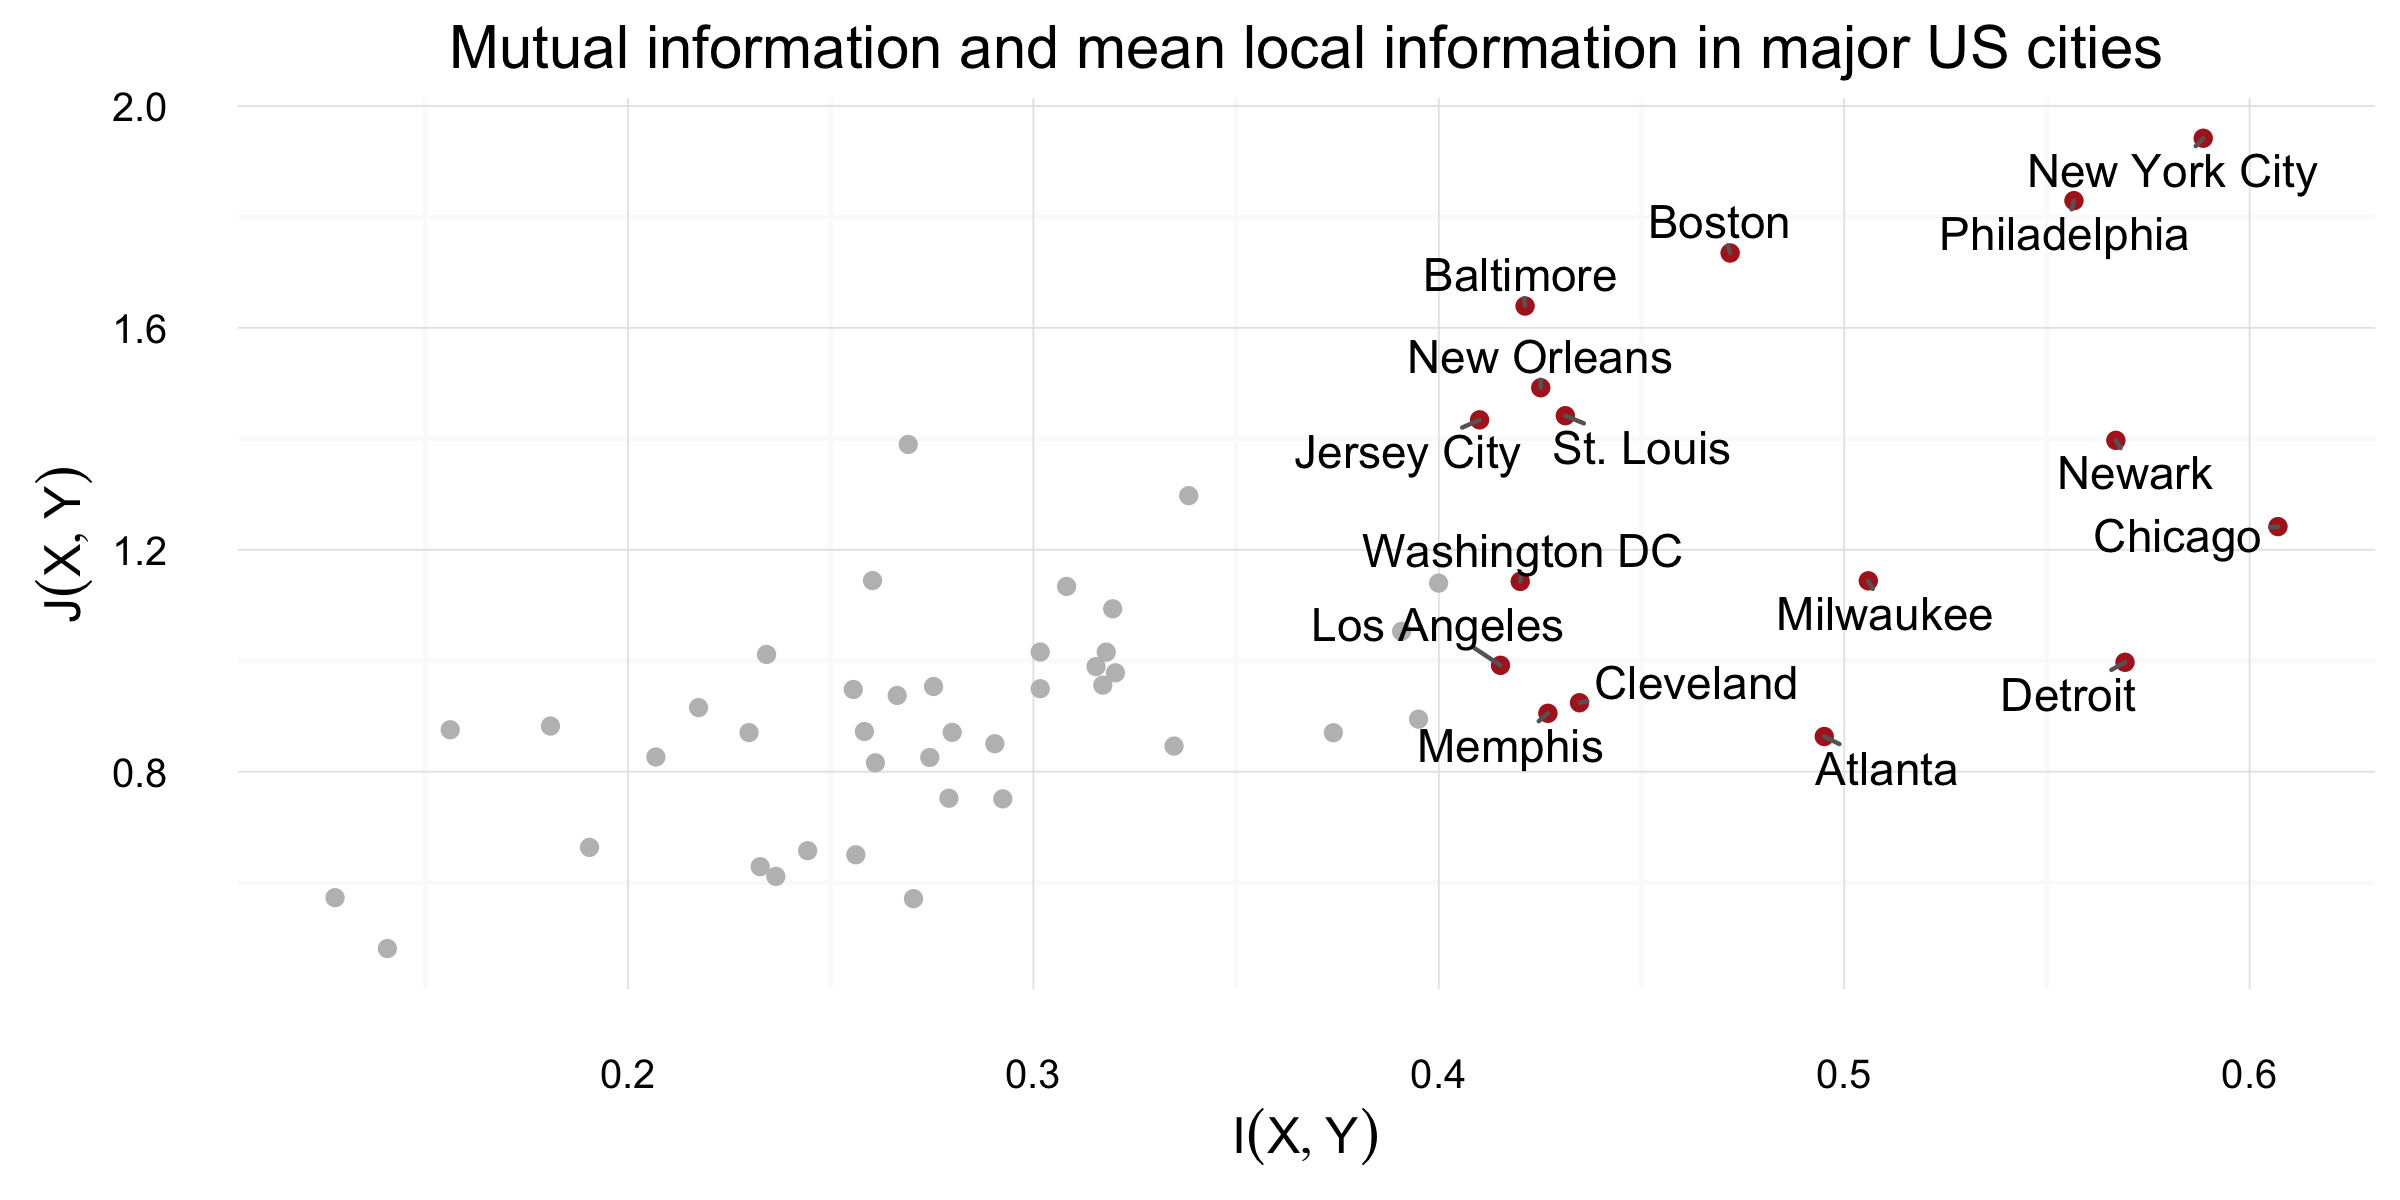
\includegraphics[width=1\textwidth]{figs/mutual_fisher.png}
			\caption{Relationship of global mutual information $I(X,Y)$ and mean local information $J(X,Y)$.} 
			\label{fig:info_cross}
		\end{figure}	
	Figure \ref{fig:info_cross} shows the relationship of the global spatial variability $I(X,Y)$ and mean local variability $J(X,Y)$. An overall positive trend is evident, reflecting the fact that global spatial variability is a prerequisite for local variability: if the city is uniform (like Figure \ref{fig:toy}(a)), then no local differences either exist.  On the other hand, there are substantial variations in $J(X,Y)$ even in cities with comparable global variability $I(X,Y)$. For example, the cities of Detroit and Philadelphia provide a striking contrast. While they have comparable global variability $I(X,Y)$, Philadelphia's $J(X,Y)$ is substantially higher. This reflects the fact that Detroit is composed of large, highly-segregated, monoracial neighborhoods, whereas Philadelphia has a much more fine-grained, intricate neighborhood structure. These patterns illustrate how combinations of the information measures $H(Y)$, $I(X,Y)$, and $J(X,Y)$ can be used to construct taxonomies diversity for American cities. 

	Intriguingly, the mean local variability $J(X,Y)$ appears obey a scaling relation with respect to urban density. In Figure \ref{fig:density}, we plot $J(X,Y)$ against the population density $\rho$ of our studied cities. A clear trend is evident, with $J(X,Y)$ growing linearly with the logarithm of density. We interpret this trend as reflecting a compression of social space in dense urban areas: the same structure of racial variability fits into much less geographical area in New York than in Phoenix. One aspect of diversity in large, dense cities is that one need walk much less distance in order to reach a neighborhood with substantially different racial trends than one's own. 
	 
		\begin{figure}
			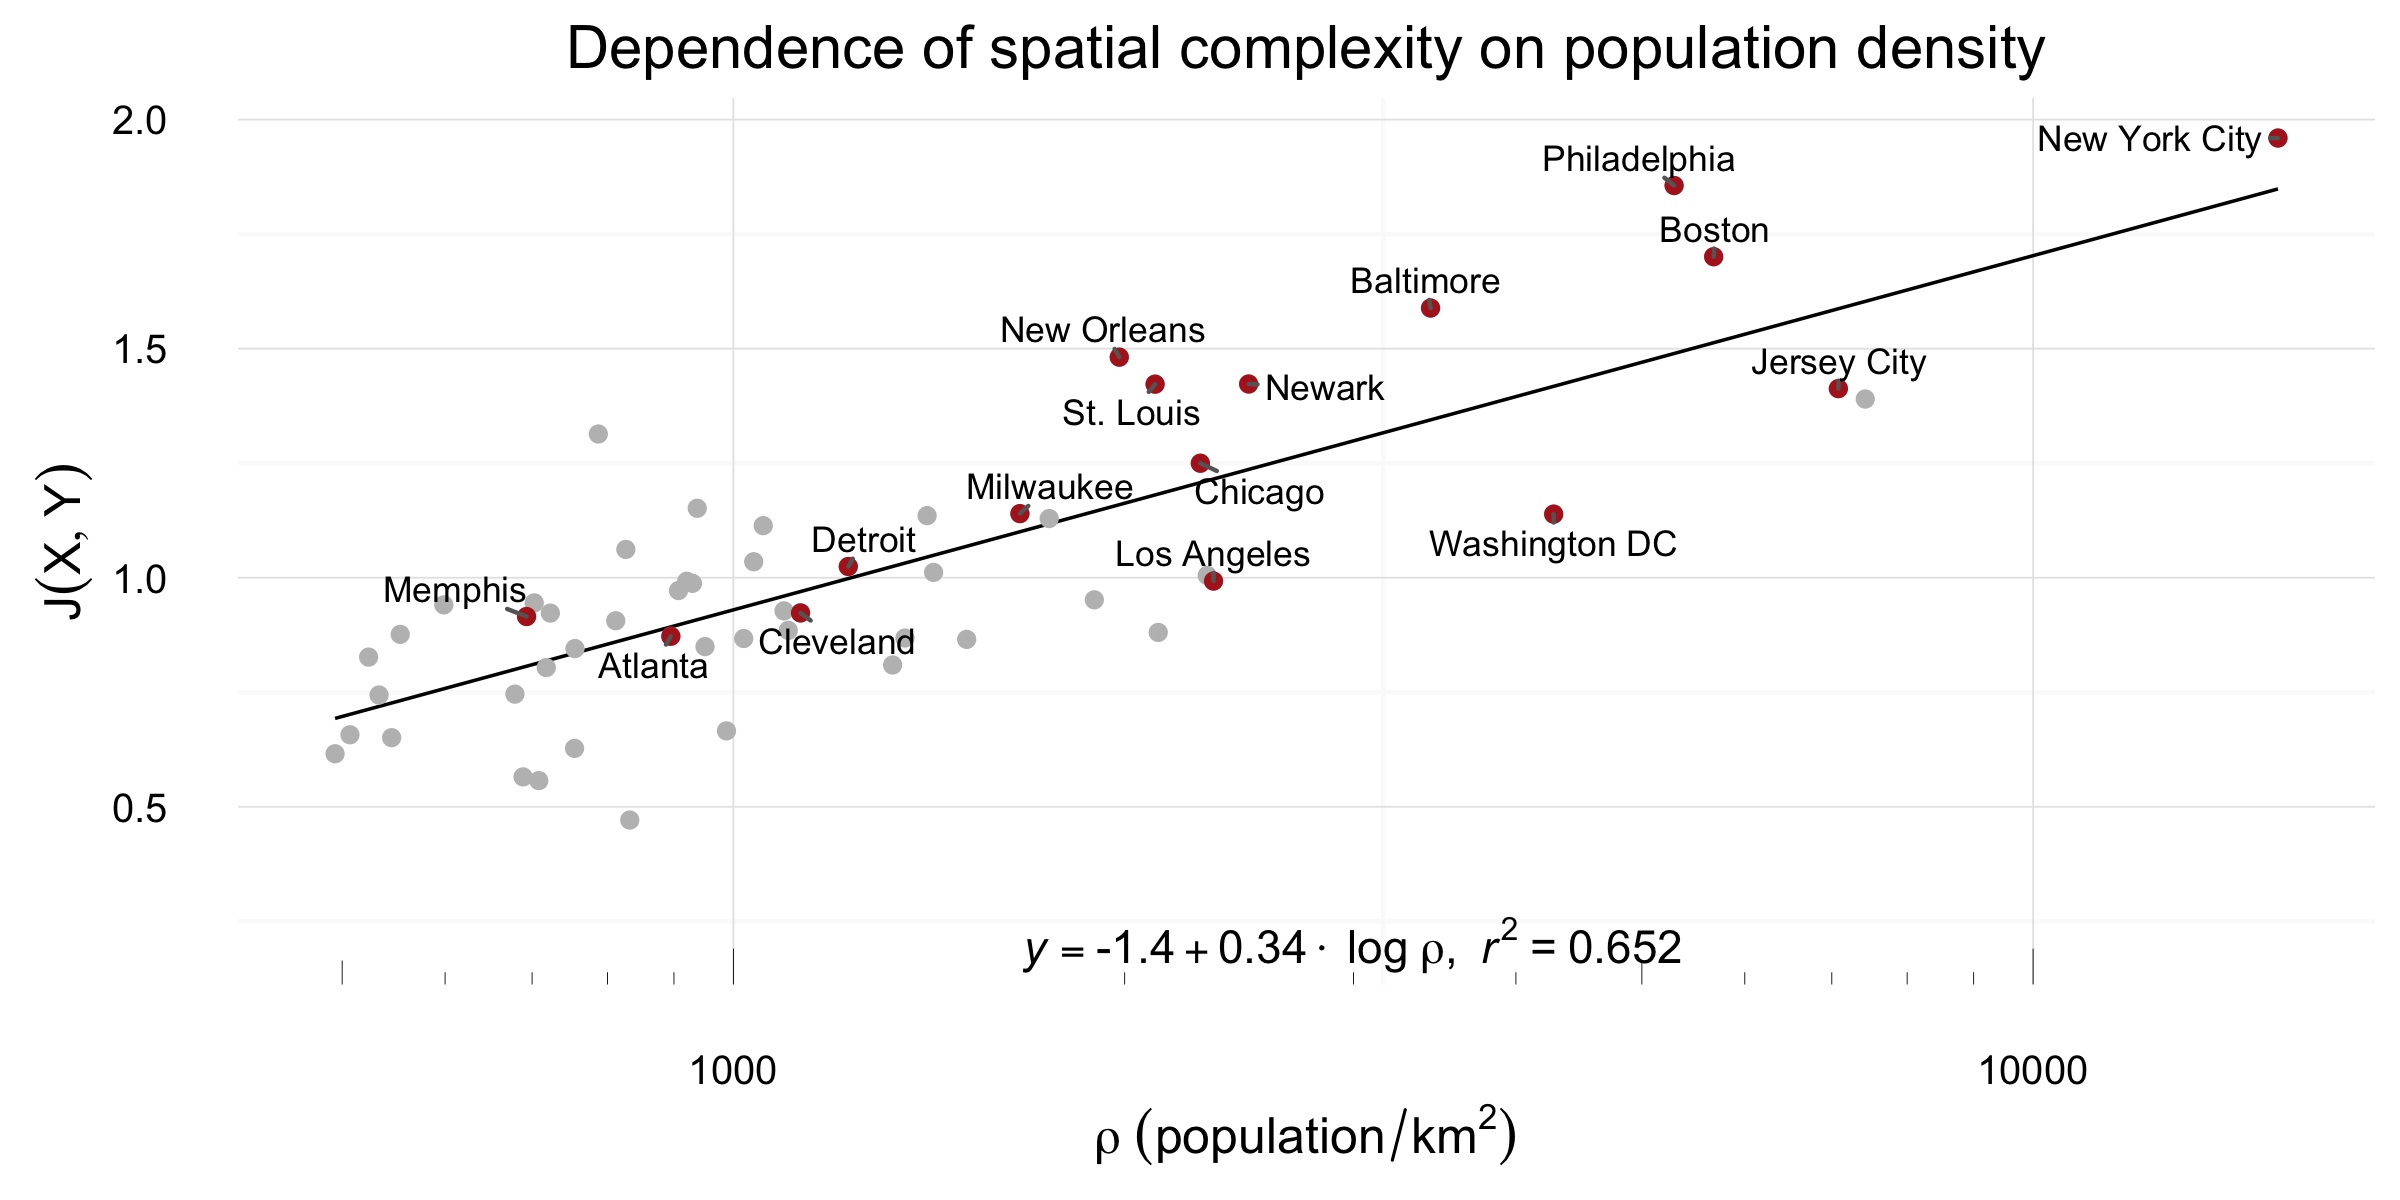
\includegraphics[width=1\textwidth]{figs/density_fisher.png}
			\caption{The mean local information $J(X,Y)$ scales with the logarithm of population density.}
			\label{fig:density}
		\end{figure}	

\subsection{Complexity and Neighborhood Identification}


	Figure \ref{fig:cluster_map} shows an illustrative clustering into ten regions according to equation \eqref{eq:info_dist} for the city of Chicago. 
	
		\begin{figure}
			\centering
			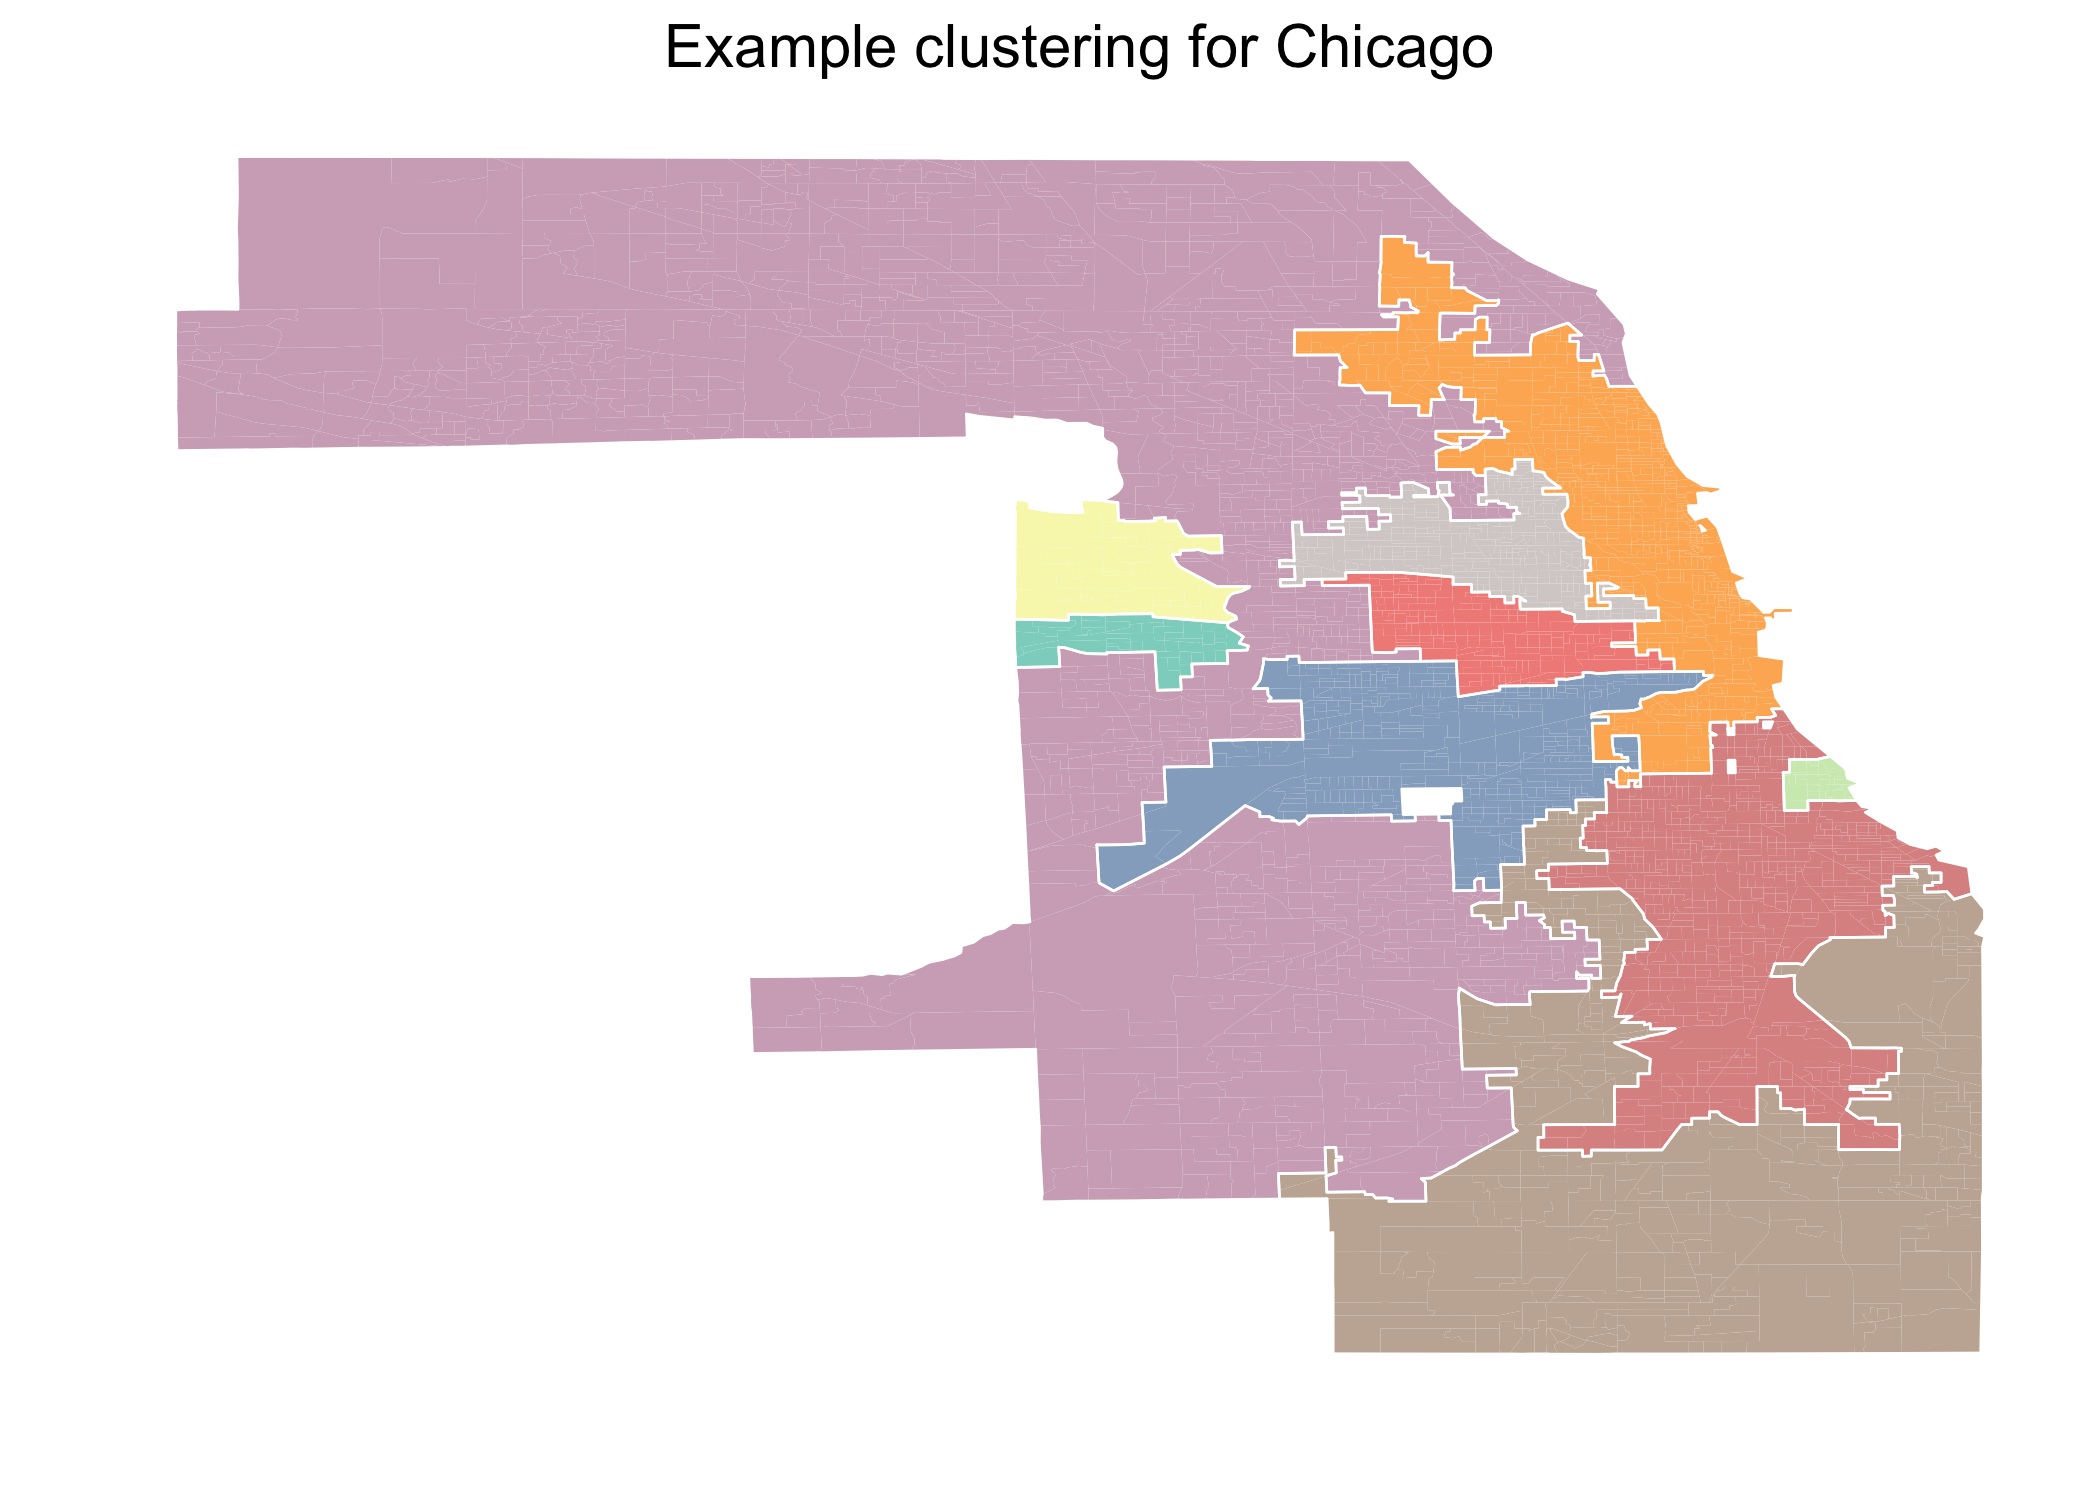
\includegraphics[width=\textwidth]{figs/example_cluster_map.png}
			\caption{The regions determined by our hierarchical clustering algorithm reflect high-level racial trends across space. The clusters on the right sharply segment predominantly Black, Hispanic, and White neighborhoods in Central Chicago.}
			\label{fig:cluster_map}
		\end{figure}		

		We expect that spatially complex cities with high $J(X,Y)$ would require more complicated models in order to convey similar amounts of demographic information. Testing this expectation requires a quality measure defined on cluster models for each city. The natural measure of loss for a clustering is the mutual information $I(C,Y)$ between cluster and racial labels. Cities vary sharply in the level of cluster detail needed to convey equal amounts of information about race, as shown in figure \ref{fig:clusters}. Each clustering has approximately equal $I(C,Y)$. In sharply segregated Atlanta, just two clusters--one predominantly white, the other predominantly black--suffice to convey more information than do five in Boston, where the clusters are substantially more nuanced. Cluster 1 is predominantly white, cluster 4 majority Hispanic, and cluster 5 overwhelmingly black. Cluster 2 is again majority white, but is unique in that its minority citizens are almost all Hispanic, while cluster 3 is approximately equally black and Hispanic. 

		These clusterings can also reveal phenomena related to traditional concepts in segregation studies, such as affinity and concentration. In Figure \ref{fig:clusters}, across all cities, Asians are much more likely to be found in predominantly white clusters than they are in predominantly black or Hispanic ones, indicating significant spatial integration between these two groups. We can observe the phenomenon of concentration -- in which marginalized groups tend to be more highly concentrated in their regions than majority groups are in theirs -- in Atlanta and Detroit. In Atlanta, whites make up 61\% of cluster 1, while blacks make up 83\% of cluster 2. Similarly in Detroit, whites make up 70\% of cluster 1, while blacks make up a full 86\% of cluster 2. 

		\begin{figure}
			\centering
			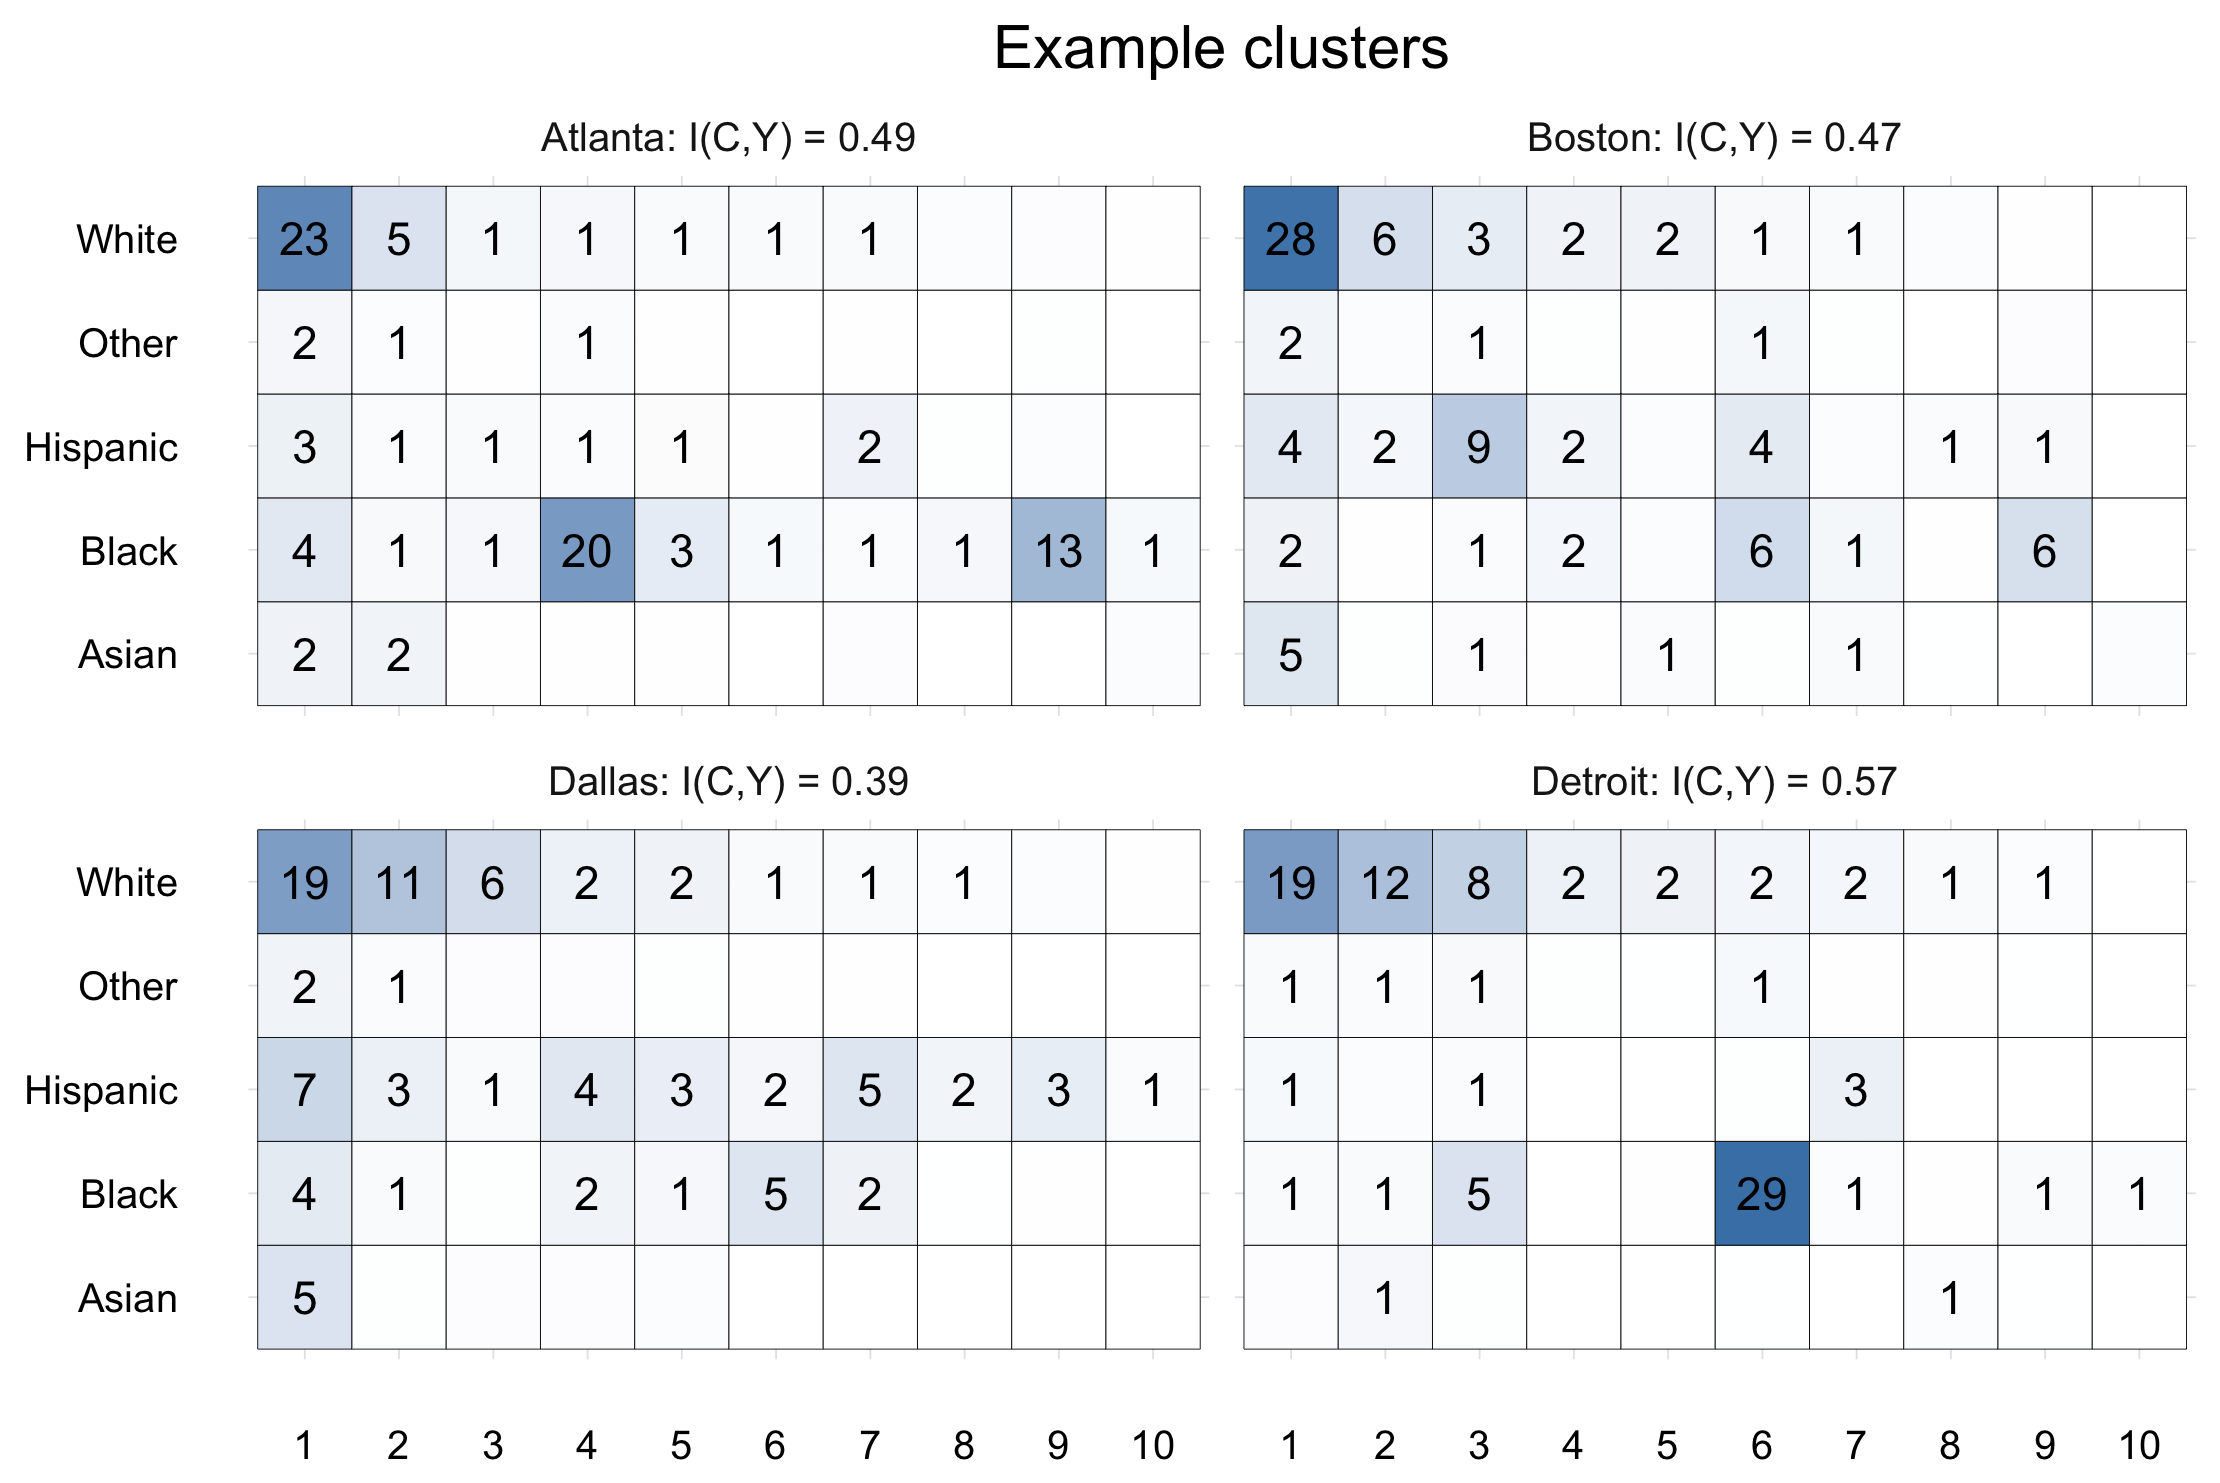
\includegraphics[width=\textwidth]{figs/example_clusters.png}
			\caption{Example clusters for different cities, and the associated mutual information contained in each. The number in each box reflects the percentage of the population in the labeled racial group and cluster. }
			\label{fig:clusters}
		\end{figure}		

		To develop a global evaluation of the hierarchical clustering of a city according to the method defined by \eqref{eq:info_dist}, we borrow the methodology of the ``area under the curve'' (AUC) used extensively in statistical learning. By plotting the information $I(C,Y)$ against the number of clusters $n$, we obtain a curve reflecting how the information evolves at varying scales of aggregation. Figure \ref{fig:AUC} illustrates these curves for Boston and Detroit, with $N$ plotted on a logarithmic scale.  

		\begin{figure}
			\centering
			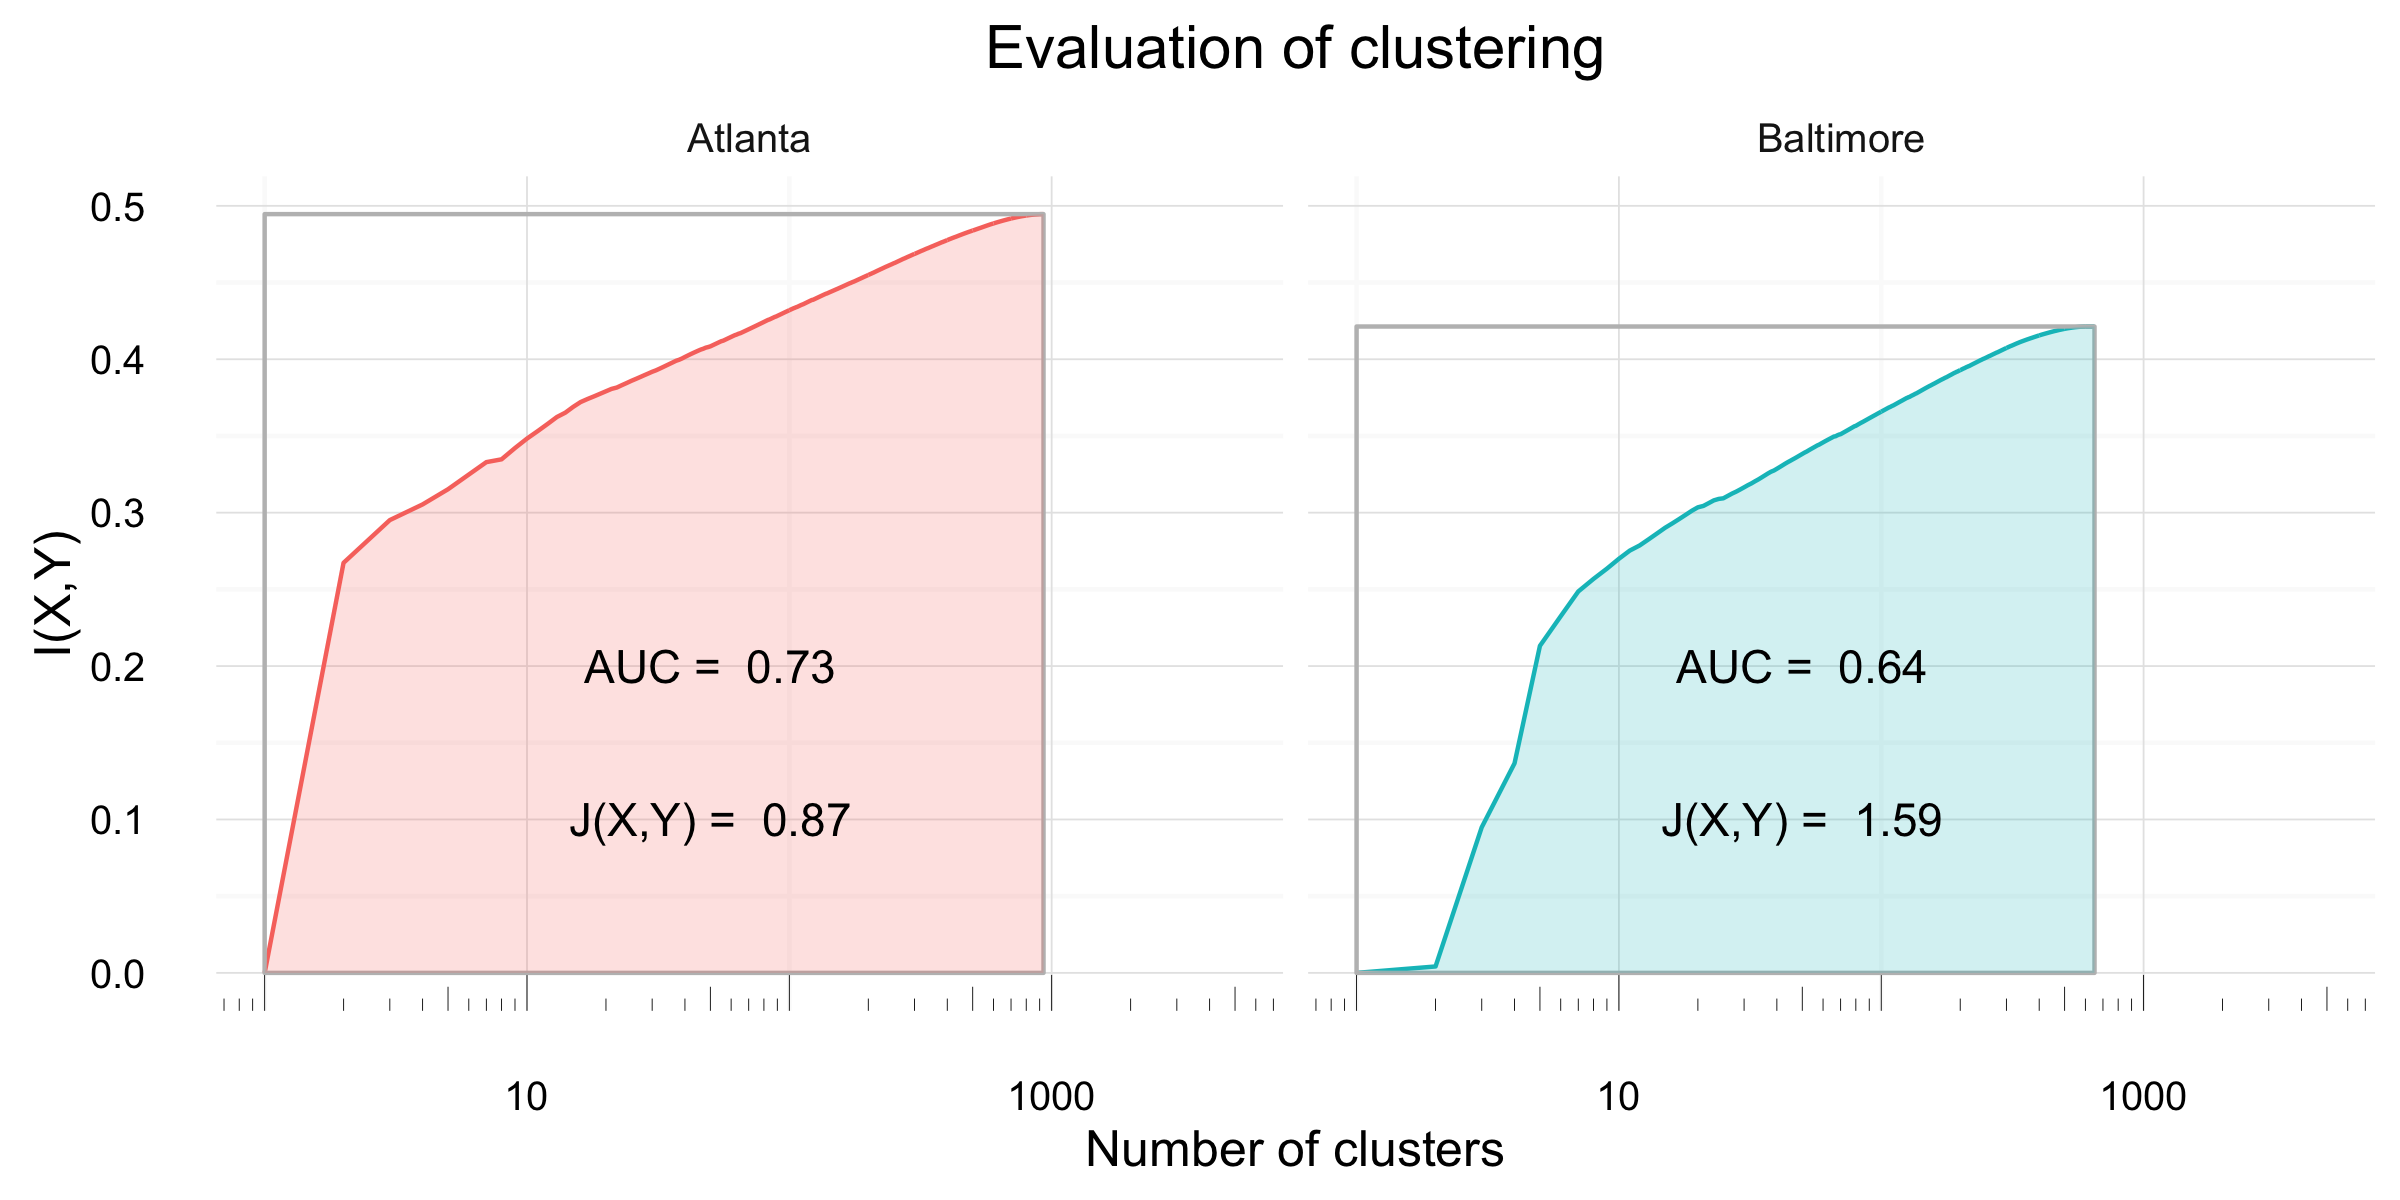
\includegraphics[width=\textwidth]{figs/AUC_illustration.png}
			\caption{Evaluation of clustering using an Area Under the Curve (AUC) metric. The AUC is the fraction of the bounding box lying under the information gain curve. Boston's AUC is smaller than Detroit's, showing that Boston's spatial complexity (measured by $J(X,Y)$) requires more complex models than Detroit's.}
			\label{fig:AUC}
		\end{figure}

		Figure \ref{fig:AUC} also shows the bounding rectangle, whose top right corner is defined by the number N of tracts in the census data set and the full mutual information $I(X,Y)$. The AUC is defined as the ratio of the shaded area in Figure \ref{fig:AUC} to the bounding rectangle. An AUC of 1 indicates that just one region carries full information; this can only occur in a city with no spatial variation, such as city (b) in \ref{fig:toy}. A larger AUC indicates that sample models with few regions capture more information about spatial variation in the city. In Detroit, there exists a clear dividing line between a predominantly white region on the west and a predominantly black region in the east. A two-cluster model therefore captures much of the information in the city, giving a high AUC of 0.74. In Boston, on the other hand, no such clear divide exists, and more complex models are necessary to capture similar amounts of information. Thus, Boston has a lower AUC of 0.67. 

		\begin{figure}
			\centering
			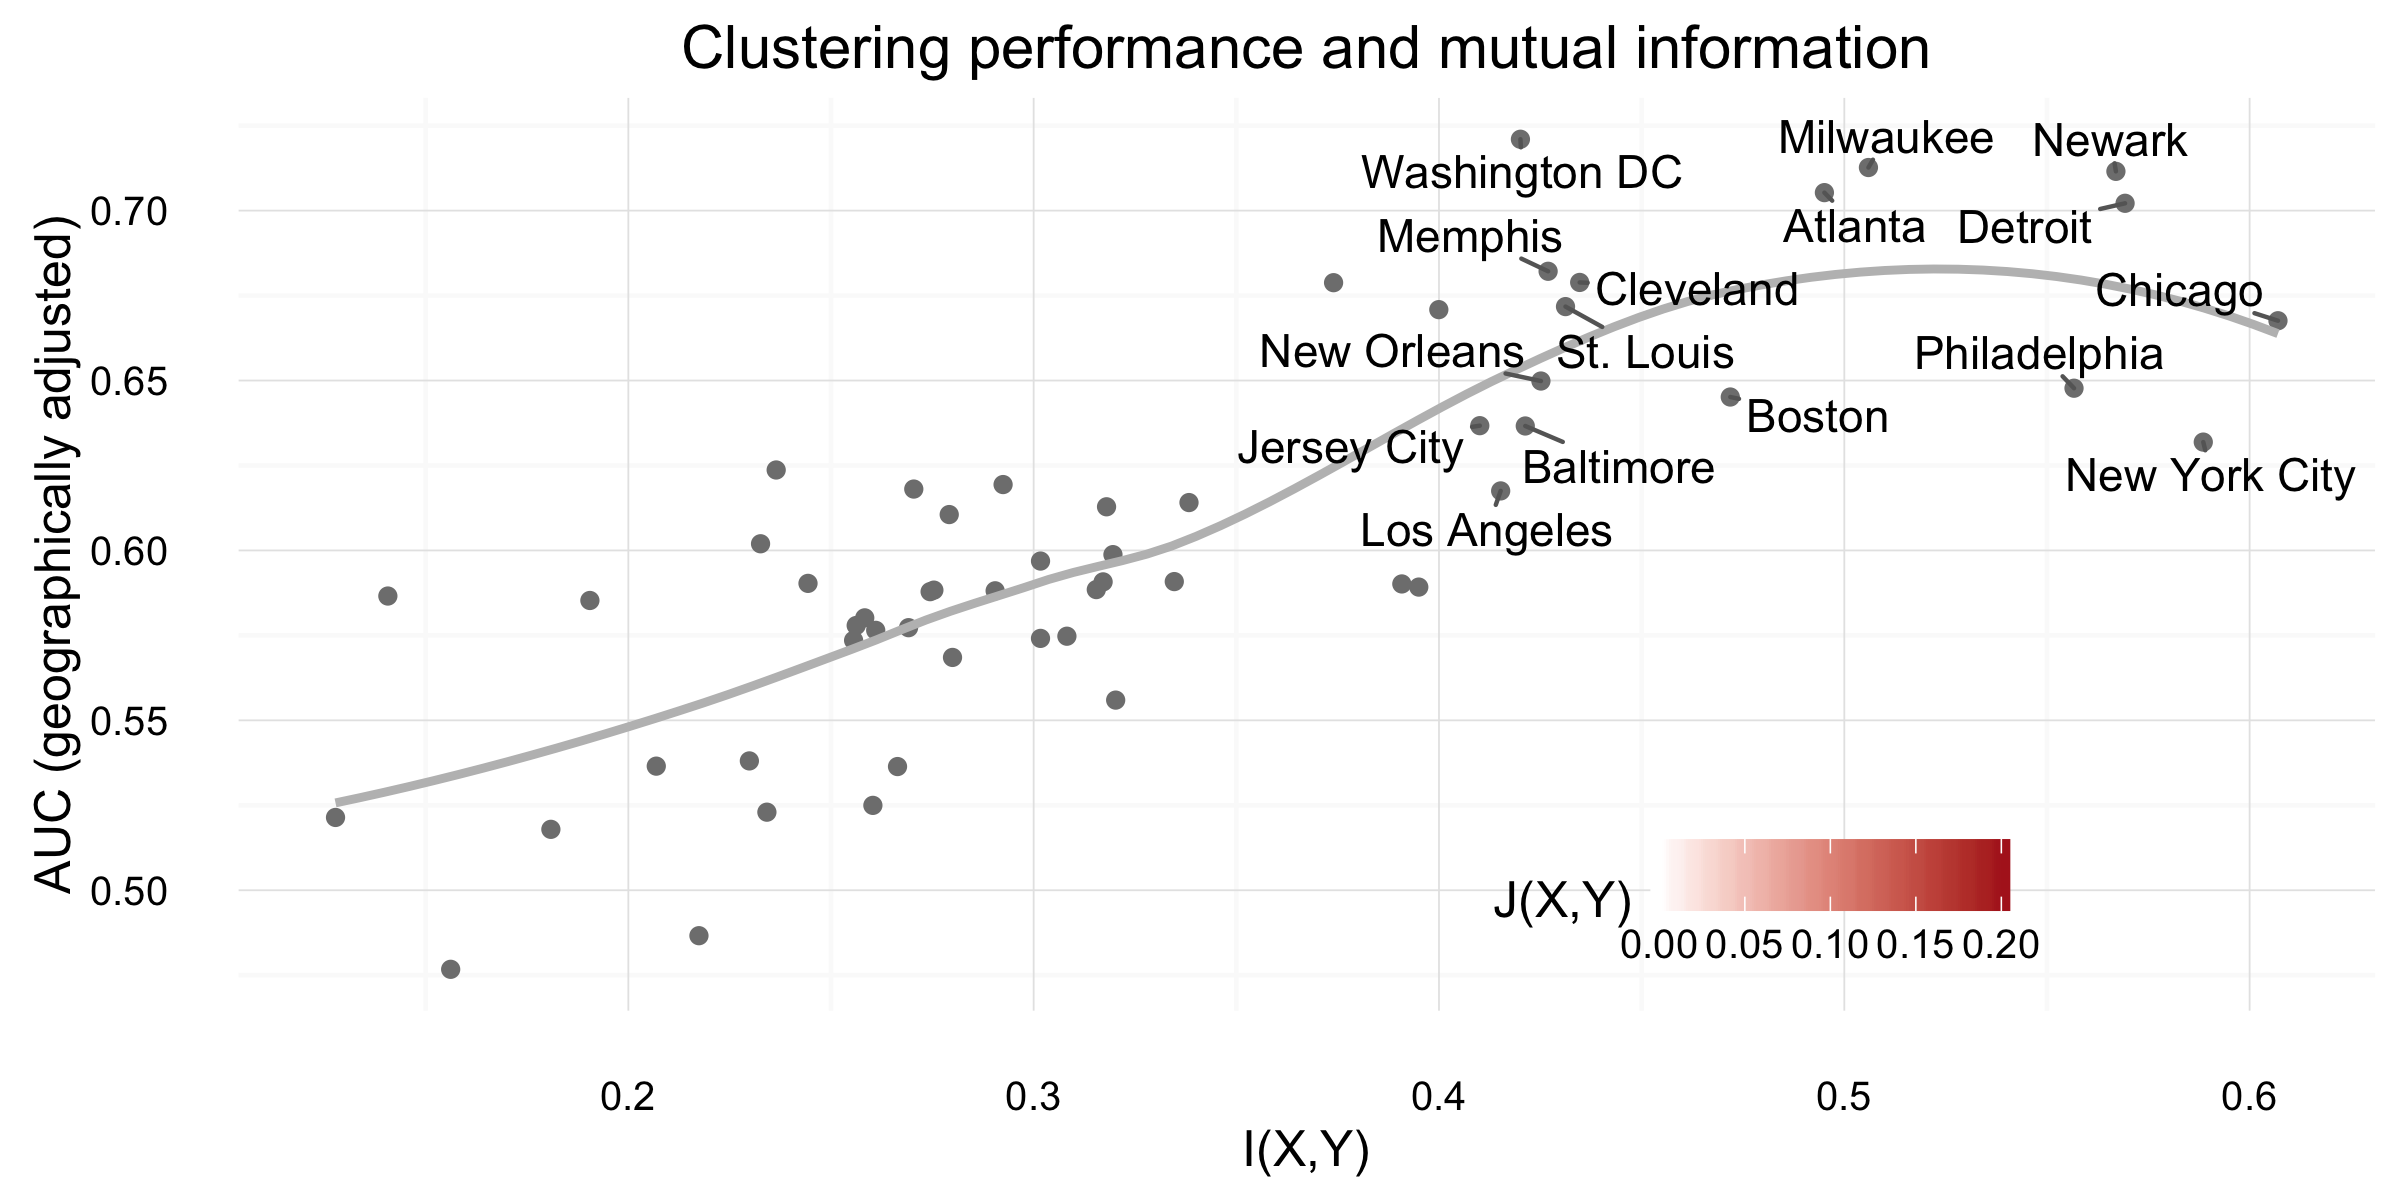
\includegraphics[width=\textwidth]{figs/info_performance_adjed.png}
			\input{figs/adjusted_regression.txt}

			\caption{Relationship between information measures $I(X,Y)$, $J(X,Y)$, and the clustering AUC. The AUC has been geographically adjusted to account for cities like New York, whose Census blockgroups form eight disconnected components, which would mildly distort results without adjustment. Table produced using \cite{Marek2015}}.
			\label{fig:info_and_clusters}
		\end{figure}		

		Based on our discussion so far, we would expect that the AUC is related to the information measure $J(X,Y)$. Figure \ref{fig:info_and_clusters} confirms this expectation. Overall, two factors explain much about the ``clusterability'' of a city as measured by the AUC. The most important factor is the overall mutual information $I(X,Y)$. This reflects a simple intuition: when there is little spatial variation, there is not much to cluster. The second factor is the mean local information $J(X,Y)$, reflecting that spatial complexity makes clustering harder. A simple linear regression makes these insights precise. As predictors of the AUC, both $I(X,Y)$ and $J(X,Y)$ are highly significant, and the coefficient of $J(X,Y)$ is negative. The two measures jointly account for an adjusted 72\% of the variation in AUC. 